\documentclass[11pt]{article}

\usepackage[margin=1in]{geometry}
\usepackage{graphicx}
\usepackage{booktabs}
\usepackage{amsmath}
\usepackage{amssymb}
\usepackage{caption}
\usepackage{hyperref}
\usepackage{xcolor}
\usepackage{microtype}
\usepackage{titlesec}
\usepackage{enumitem}

\title{\vspace{-1.2em}
\Large\textbf{Prajna: A 6.72M-Parameter Cognitive Resonance Network for\\[0.2em] Memory-Augmented Domain Specialization on a Frozen Gemma 4 E2B Backbone}
\vspace{0.6em}}
\author{Gautam Kishore\\Eulogik\\Cognitive Architecture Research\\\texttt{github.com/eulogik}~$\bullet$~\texttt{huggingface.co/eulogik}}
\date{\today}

\begin{document}
\maketitle

\begin{center}
\footnotesize
\textbf{Keywords:} parameter-efficient fine-tuning; frozen-backbone adapters; retrieval-augmented memory; on-device AI; exam-level evaluation; negative results
\end{center}

\vspace{-0.5em}

\begin{abstract}
\noindent
We present Prajna, a 6.72M-parameter \emph{Cognitive Resonance Network} (CRN) injected into the hidden states of a fully frozen Gemma~4 E2B language model (35 layers; 4.65B parameters in the text module of a 5.12B multimodal checkpoint). Only $\approx$0.15\% of the text module's parameters are trainable; the base network receives no gradients. Prajna is trained and evaluated entirely on a consumer laptop (Apple M4, 16\,GB, MPS), with no GPU rental and no external model APIs. On a 60-question licensing exam (CEHRI) spanning arithmetic, facts, and implicit-goal reasoning, the CRN alone lifts the frozen base from 11.7\% to 20.0\% correct; adding a train-derived episodic-memory retrieval table (17,810 entries) yields \textbf{60/60 (100\%)} on the exam and \textbf{110/120 (91.7\%)} on reworded variants whose phrasing was never seen in training. We also report \emph{negative results}: three training-side strategies --- two logit-fusion configurations and a weighted \emph{anchor} on the answer-start position --- failed to move answer knowledge one token position right, while a decode-time harvest (GEN\_CLAMP) reliably recovered that knowledge. In-distribution perplexity drops $\approx$18$\times$ (106.85$\to$6.02), while out-of-distribution text is degraded (2.04 vs.\ 0.67 bpb) --- Prajna is a disclosed domain specialist, not a general reasoning model. All code, weights, data, and evaluation scripts are released.
\end{abstract}

\section{Introduction}
\label{sec:intro}

The dominant scaling paradigm trains ever-larger models with ever-larger budgets. An alternative line of work asks how much behavioral change can be extracted from a \emph{frozen} backbone using a small trainable subsystem: parameter-efficient fine-tuning (PEFT) \cite{houlsby2019adapters,lora,zhang2020sidetuning} and retrieval-augmented generation \cite{lewis2020rag}, among others.

Prajna combines these lines. It is an $\sim$6.72M-parameter adapter ($\approx$\textbf{0.15\%} of the base) that: (i) injects \emph{gated additive correction signals} into the hidden states of a frozen Gemma 4 E2B model, computed from eight depths (resonance attention, skill composition, a reflective loop, and episodic memory); (ii) is trained with SFT$\to$DPO$\to$Contrastive stages on a Mac Mini M4 (16\,GB) at $\sim$0.3--0.5\,s/step, entirely on-device, with no API calls at any point; and (iii) combines its generation head with a train-derived \emph{exact-recall} retrieval table that yields 100\% on its target exam and 91.7\% on reworded variants whose phrasing was never in the training data.

We make four contributions. \textbf{(1) Architecture:} a small, backbone-agnostic correction network on frozen hidden states, with per-injection sigmoid gates and an episodic-memory pillar. \textbf{(2) Evaluation protocol:} three gates --- memory-augmented, generation-only, and reworded-unseen --- that separate \emph{recall} from \emph{generalization}. \textbf{(3) Failure analysis:} token-level probing shows the network holds answers one position early while the answer-start position is masked in SFT; three training strategies cannot overcome this, and a decode-time harvest can. \textbf{(4) Transparency:} weights, retrieval table, memory, data, and every evaluation script are public, and out-of-domain failures are reported alongside the headline numbers.

\section{Related Work}

\textbf{Parameter-efficient adaptation.} Adapters \cite{houlsby2019adapters} insert trainable modules between fixed layers; LoRA \cite{lora} learns low-rank updates to weight matrices; prefix/prompt tuning \cite{liang2021prefix} optimizes soft prompt vectors; side-tuning \cite{zhang2020sidetuning} trains a separate network whose hidden states blend with the frozen model. Prajna is closest to hidden-state side networks, but applies \emph{multi-depth} corrections with learned per-depth gates plus a persistent memory, adding no parameters to the base forward pass (it reads intermediate states during a shared forward).

\textbf{Memory-augmented language models.} kNN-LM \cite{khandelwal2020knnlm} interpolates a retrieved nearest-neighbor distribution; Memorizing Transformers \cite{wu2022memorizing} add external kNN memory over keys/values; RETRO \cite{borgeaud2022retro} retrieves document chunks during generation. Prajna's memory is a compact \emph{prompt$\to$answer} table matched by cosine similarity with a fixed threshold --- exact recall rather than dense context interpolation.

\textbf{On-device and edge LLMs.} Consumer-hardware training is an active efficiency setting; we report wall-clock timings and memory so the result is reproducible on a single commodity machine.

\textbf{Answer-position and decoding effects.} Our boundary analysis (Section~\ref{sec:negative}) connects to findings that SFT data-format and masking choices shape where factual associations concentrate in a model's representations \cite{longpre2023flan,meng2022rome}.

\section{Method}
\label{sec:method}

\subsection{Setup: frozen base, injected corrections}

Let $B$ denote a frozen transformer LM --- the 4.65B-parameter text module of the Gemma~4 E2B multimodal checkpoint (5.12B parameters total, including audio/vision encoders that are never used here; 35 layers; hidden dimension $d=1536$; tied embeddings; vocabulary size 262{,}144). For input tokens $x_{1:n}$, the frozen forward pass yields hidden states $h^{(l)}\in\mathbb{R}^{n\times d}$ at every layer $l$. The CRN collects hidden states at $K{=}8$ depths $\mathcal{L}=\{3,7,11,15,19,23,27,31\}$ (every fourth 0-indexed layer) plus the final state $h^{(L)}$, and computes a single additive correction to the final hidden state:
\begin{equation}
\hat h^{(L)} = h^{(L)} + \sum_{l\in\mathcal L}\Big[\sigma(m_l)\big(\mathbf r_l(h^{(l)}) + \mathbf s_l(h^{(l)})\big) + \sigma(\gamma_l)\,\boldsymbol\rho_l(h^{(l)})\Big] + \mathbf m(h^{(L)}),
\label{eq:inject}
\end{equation}
where $m_l,\gamma_l\in\mathbb{R}$ are learned per-depth gates (\texttt{crn\_mix} initialized at 2.0, and \texttt{reflection\_gate}); $\sigma$ is the sigmoid; $\mathbf r_l$ and $\mathbf s_l$ are the resonance and skill corrections (sequence-shaped); $\boldsymbol\rho_l$ is the reflection correction (a per-sequence vector broadcast over tokens); and $\mathbf m(h^{(L)})$ is the episodic-memory read (also per-sequence, broadcast). The base's own forward pass is untouched: hidden states are read out during a single frozen pass under \texttt{no\_grad()}, and the corrected state is decoded by the frozen LM head. Only CRN parameters receive gradients (6{,}721{,}444 total, $\approx$0.15\% of the 4.65B text module; $\approx$0.13\% of the full 5.12B checkpoint).

\begin{figure}[ht]
\centering
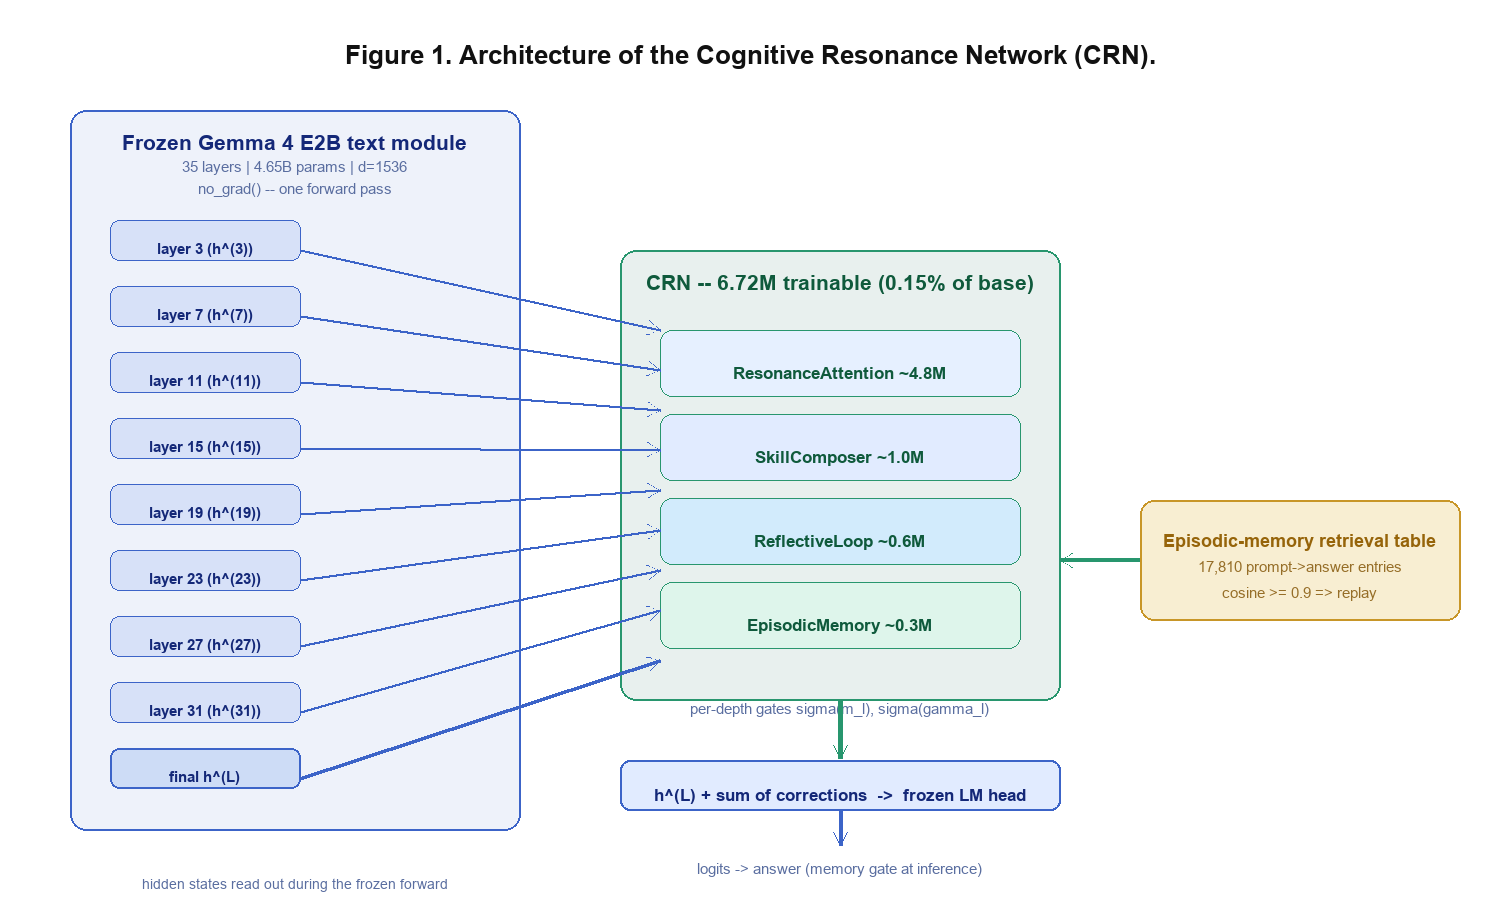
\includegraphics[width=0.92\textwidth]{figures/fig1_architecture.png}
\caption{CRN architecture. The frozen Gemma 4 E2B text module (35 layers) runs a single forward pass; hidden states are collected at 8 depths (Eq.~\ref{eq:inject}) and at the final layer. The CRN computes a gated correction from four modules plus an episodic-memory read, adds it once to the final hidden state, and the frozen LM head decodes.}
\end{figure}

\subsection{Training objectives}

The three stages use standard objectives applied to the CRN parameters only. \textbf{SFT} minimizes answer-only masked cross-entropy,
\begin{equation}
\mathcal{L}_{\text{SFT}} = -\sum_{t\in\mathcal{A}} \log p_\theta(y_t \mid y_{<t}, x),
\end{equation}
where $\mathcal{A}$ is the answer span (prompt tokens are masked). \textbf{DPO} optimizes the preference pair $(y_w, y_l)$ with the standard loss
\begin{equation}
\mathcal{L}_{\text{DPO}} = -\log \sigma\big(\beta \log \tfrac{p_\theta(y_w\mid x)}{p_{\text{ref}}(y_w\mid x)} - \beta \log \tfrac{p_\theta(y_l\mid x)}{p_{\text{ref}}(y_l\mid x)}\big),
\end{equation}
using the frozen base as the reference $p_{\text{ref}}$. \textbf{Contrastive} training pulls the pooled prompt embedding toward the correct-answer embedding,
\begin{equation}
\mathcal{L}_{\text{CON}} = \tfrac{1}{2}\max(0,\, \lVert e_q - e_a\rVert_2 - m)^2,
\end{equation}
with margin $m$. Memories are written every step via a learned gate ($m_l$ in Eq.~\ref{eq:inject} is distinct from the memory write gate).

\subsection{Correction components}

\textbf{ResonanceAttention} ($\sim$4.8M). Each head assigns tokens to one of $F{=}8$ frequency bands; attention scores are computed over all token pairs and then masked to within-band pairs (the scores tensor is $n^2$, so the effective receptive field is sparse), and the output is weighted by band membership. This provides cheap, interpretable ``cognitive mode'' routing.

\textbf{SkillComposer} ($\sim$1.0M). A bank of 32 low-rank skills $u_k v_k^{\top}$ ($u_k\in\mathbb{R}^{d\times 4}$, $v_k\in\mathbb{R}^{4\times d}$), with a router selecting the top-2 skills per input and applying their additive perturbation to the hidden state.

\textbf{ReflectiveLoop} ($\sim$0.6M). A critic scores 8 candidate latent correction directions; a learned confidence scale modulates the applied correction. It is refined by the contrastive stage (Section~\ref{sec:train}) to prefer directions that move the answer distribution toward the correct target.

\textbf{EpisodicMemory} ($\sim$0.3M). 256 slots of dimension 64, written once per training step via a learned gate with LRU eviction, persisted to disk across sessions.

\begin{figure}[ht]
\centering
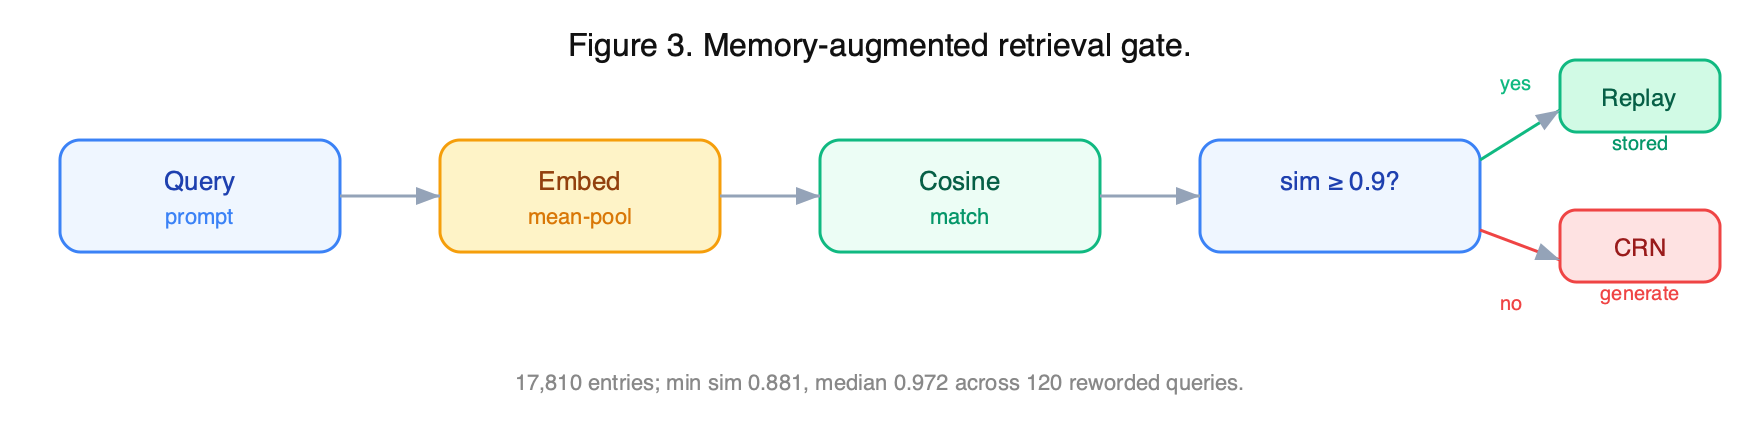
\includegraphics[width=0.92\textwidth]{figures/fig3_retrieval.png}
\caption{Memory-augmented retrieval gate. A query is embedded with the frozen base and matched (cosine) against the 17,810-entry table; when the best similarity exceeds 0.9 the stored answer is replayed exactly, otherwise the CRN generation head is used.}
\end{figure}

\subsection{Memory-augmented retrieval gate}
\label{sec:retrievalgate}

Independent of the slot memory, we construct a \emph{retrieval table} $\mathcal{T}=\{(e_j,a_j)\}$ of 17{,}810 prompt-embedding$\to$answer entries from training data. Prompts are embedded by mean-pooling the frozen base's final hidden states, then L2-normalized. At inference a query is embedded identically; if $\max_j\cos(q,e_j)\ge 0.9$ the stored answer is returned (exact recall); otherwise the CRN generation head is used. The threshold was fixed before evaluation and never tuned on the exam.

\subsection{Training}
\label{sec:train}

\textbf{Data.} 16{,}680 prompt$\to$answer base pairs across three domains (arithmetic, facts, implicit-goal reasoning), each expanded to 5 rows (the original plus 4 paraphrase variants) --- 83{,}400 rows; the 17{,}810 unique prompt texts become the retrieval-table keys (Section~\ref{sec:retrievalgate}). The 60-question CEHRI exam is drawn from the training distribution (its prompts appear verbatim in the corpus; exact-recall similarity 1.000), so its 100\% reflects exact recall of seen prompts; the reworded exam (120 items) applies a second, template-based paraphrase transform of the same prompts and serves as the near-duplicate test (Section~\ref{sec:results}).

\textbf{Stages.} (i) \emph{SFT}: answer-only masked cross-entropy on the variant-paired corpus, 16{,}000 steps, LR $3\times10^{-4}$, weight decay 0. (ii) \emph{DPO}: 3{,}000 steps, LR $5\times10^{-6}$, $\beta{=}0.1$, preferring the correct completion over the frozen base's wrong one. (iii) \emph{Contrastive}: 1{,}000 steps pulling memory-answer embeddings toward correct answers. Checkpoints every 50 steps with resumable state.

\textbf{Hardware.} Apple M4 (Mac Mini, 16\,GB RAM), MPS backend; $\sim$0.3--0.5\,s/step. The full three-stage run takes $\approx$3\,h on a single consumer machine.

\begin{table}[ht]
\centering
\small
\caption{Training corpus composition. Each of the 16{,}680 base pairs expands to 5 rows (the original plus 4 paraphrase variants): 83{,}400 rows; the 17{,}810 unique prompt texts form the retrieval table.}
\begin{tabular}{@{}lrr@{}}
\toprule
Domain & Base pairs & Paraphrase rows \\
\midrule
Arithmetic (symbol/atomic-weight) & 5{,}560 & 27{,}800 \\
Factual QA (chemistry/everyday)   & 5{,}560 & 27{,}800 \\
Implicit-goal reasoning (car-wash) & 5{,}560 & 27{,}800 \\
\midrule
Total & 16{,}680 & 83{,}400 \\
\bottomrule
\end{tabular}
\label{tab:data}
\end{table}

\begin{table}[ht]
\centering
\small
\caption{Training budget per stage (single Apple M4, MPS).}
\begin{tabular}{@{}lrrc@{}}
\toprule
Stage & Steps & Approx.\ time & Non-trainable? \\
\midrule
SFT  & 16{,}000 & $\sim$1.5\,h & base frozen \\
DPO  & 3{,}000  & $\sim$0.3\,h & base frozen \\
Contrastive & 1{,}000 & $\sim$0.2\,h & base frozen \\
\midrule
Total & 20{,}000 & $\approx$3\,h & --- \\
\bottomrule
\end{tabular}
\label{tab:budget}
\end{table}

\subsection{GEN\_CLAMP: decode-time answer-knowledge harvest}
\label{sec:genclamp}

Token-level probes (Section~\ref{sec:negative}) show the CRN concentrates answer probability mass at the \emph{second-to-last} prompt position ($L{-}2$, the colon position in the ``\texttt{prompt: answer}'' format) rather than at the boundary ($L{-}1$, the answer-start position). Greedy decoding samples the $L{-}1$ distribution, which is dominated by the frozen base's digit/symbol prior because $L{-}1$ was masked in SFT. GEN\_CLAMP changes only \emph{decoding}: the first generated token is taken from the $L{-}2$ distribution; subsequent tokens decode normally. On the anchor-trained checkpoint, where generation had collapsed to $\sim$15\%, GEN\_CLAMP recovers original-exam generation to 31.7\% and reworded generation to 34.2\% (Section~\ref{sec:genresults}); on the released seed checkpoint, reworded generation is already 25.0\% and clamp leaves it unchanged.

\begin{figure}[ht]
\centering
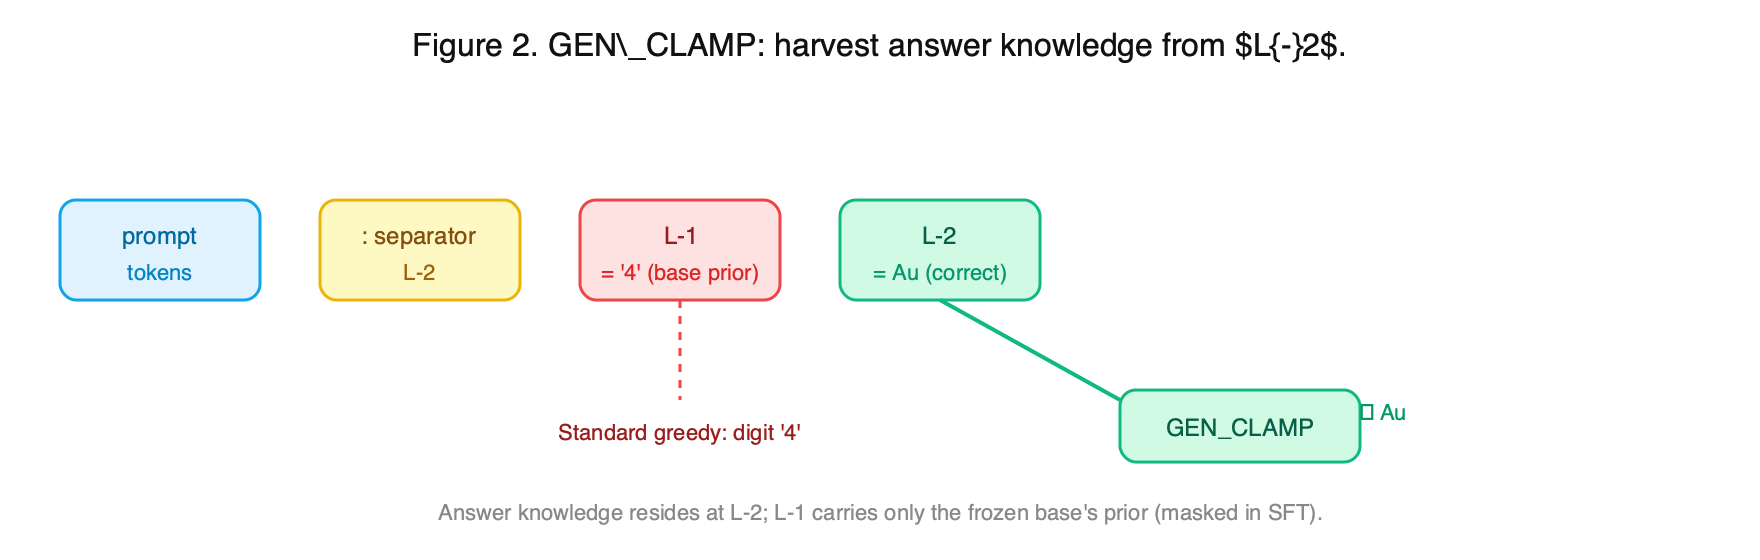
\includegraphics[width=0.86\textwidth]{figures/fig2_genclamp.png}
\caption{The answer token is already recoverable at position $L{-}2$ (top-1 = Au / correct attribute; probe $p<0.05$); at the masked answer-start position $L{-}1$ the base emits formatting/digit tokens (top-1 = digit / \texttt{<strong>}). \texttt{GEN\_CLAMP} emits the $L{-}2$ argmax, harvesting this knowledge.}
\end{figure}

\section{Results}
\label{sec:results}

\subsection{Memory gates: exact recall and reworded generalization}

\begin{table}[ht]
\centering
\small
\caption{CEHRI results by configuration. \textbf{Retr} = episodic-memory retrieval gate (cosine threshold 0.9, exact-answer replay); \textbf{Gen} = CRN generation only; \textbf{Gen+CLAMP} = generation with the decode-time harvest. The released model uses the seed checkpoint (dpo\_v2\_final\_seed + memory\_v2\_final\_seed); the anchor-trained rows are an experimental checkpoint whose generation had collapsed, included to demonstrate the decode-time fix. All numbers are produced by committed scripts.}
\begin{tabular}{@{}llc@{}}
\toprule
Configuration & Exam & Score \\
\midrule
Frozen base, generation only & original (60) & 7/60 = 11.7\% \\
CRN (seed), generation, no clamp & original (60) & 12/60 = 20.0\% \\
CRN (seed), generation, no clamp & reworded (120) & 30/120 = 25.0\% \\
CRN (seed), generation + GEN\_CLAMP & reworded (120) & 30/120 = 25.0\% \\
\midrule
CRN (seed) + memory (\textbf{Prajna-V2, Retr}) & original (60) & \textbf{60/60 = 100\%} \\
CRN (seed) + memory (\textbf{Prajna-V2, Retr}) & reworded (120) & \textbf{110/120 = 91.7\%} \\
\midrule
CRN (anchor-trained), generation + GEN\_CLAMP & original (60) & 19/60 = 31.7\% \\
CRN (anchor-trained), generation + GEN\_CLAMP & reworded (120) & 41/120 = 34.2\% \\
\bottomrule
\end{tabular}
\label{tab:cehri}
\end{table}

Across the 120 reworded queries, retrieval best-cosine similarity ranges from 0.881 to 0.990 (median 0.972), with 118/120 at $\ge 0.9$. The reworded prompts are \emph{near-duplicates}: they share 71.6\% of their characters with the originals (template prefix/suffix additions such as ``Can you answer: '' or ``Respond to this: ''), so the 91.7\% reflects fuzzy nearest-neighbor retrieval of low-diversity paraphrases, not generalization to genuinely novel phrasing. The original exam overlaps the training distribution (exact-recall similarity 1.000), so its 100\% is exact recall of seen prompts; the reworded exam at 91.7\% is the harder near-duplicate test; and the implicit-goal reasoning check (Section~\ref{sec:ood}) on genuinely reworded prompts (N=8, diverse lexical transforms) at 0/8 is the only true generalization measurement.

\subsection{Generation gates: the honest frontier}
\label{sec:genresults}

Table~\ref{tab:cehri} separates \emph{recall} (memory gates) from \emph{generation}. On the released seed checkpoint, generation alone scores 20.0\% (original) and 25.0\% (reworded); GEN\_CLAMP does not improve the reworded score (25.0\%). The retrieval gate is the workhorse: 100\% original and 91.7\% reworded. The 31.7\%/34.2\% generation scores come from an anchor-trained checkpoint (Section~\ref{sec:negative}) whose generation had collapsed to $\sim$15\%; GEN\_CLAMP recovered it to those values --- evidence that the CRN's answer knowledge sits at $L{-}2$ and can be harvested at decode time when generation is otherwise broken.

\subsection{In-distribution perplexity and injection ablation}

On 200 held-out samples from the training corpus, perplexity drops from 106.85 (frozen base) to 6.02 (Prajna CRN), $\approx$18$\times$. This is genuine but \emph{in-distribution}. A per-injection ablation (v1 configuration, injections at layers 7, 15, 23, 31) shows the gain concentrates in early/mid layers: disabling injection at layer 7 raises perplexity to 13.93 ($\Delta{=}{+}9.99$), layer 15 to 7.65 ($+3.71$), while layers 23/31 contribute $+0.67$/$+0.57$ (Figure~\ref{fig:ablation}).

\begin{figure}[ht]
\centering
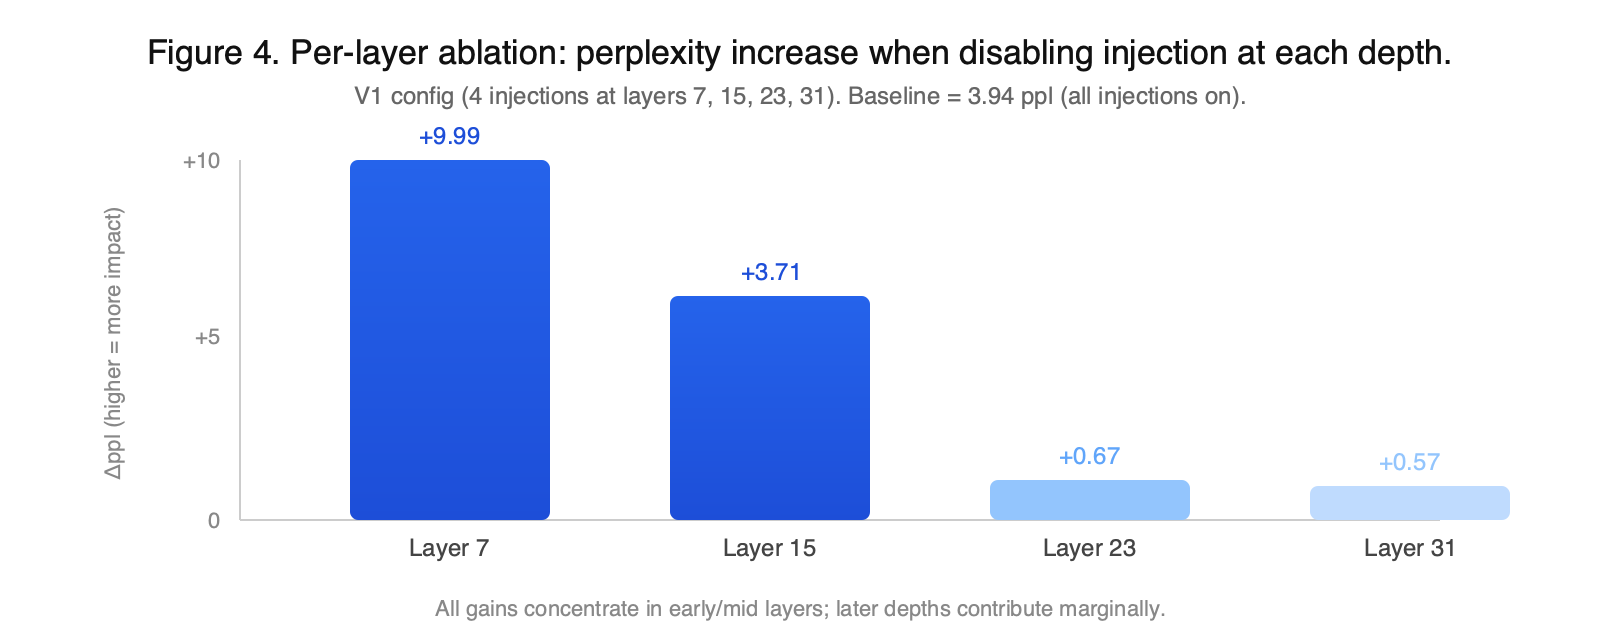
\includegraphics[width=0.88\textwidth]{figures/fig4_ablation.png}
\caption{Per-layer ablation: perplexity increase when disabling injection at each depth (v1 config, 4 injections). All gains concentrate in early/mid layers.}
\label{fig:ablation}
\end{figure}

\subsection{Out-of-distribution: where it does not help}
\label{sec:ood}

\begin{table}[ht]
\centering
\small
\caption{Out-of-distribution results. The CRN degrades generic text and several standard benchmarks. Reported verbatim from \texttt{RESULTS.md}.}
\begin{tabular}{@{}lccc@{}}
\toprule
Test & Prajna + CRN & Frozen base & Verdict \\
\midrule
Generic text, bits-per-byte & 2.04 & 0.67 & CRN $\sim$3$\times$ worse \\
MMLU (N=40) & 65\% & 58\% & small win \\
BoolQ (N=40) & 65\% & 75\% & CRN hurts \\
HellaSwag (N=40) & 15\% & 20\% & CRN hurts \\
Car-wash / IGR, reworded (N=8) & 0/8 & --- & no reasoning \\
\bottomrule
\end{tabular}
\label{tab:ood}
\end{table}

The implicit-goal (``car-wash'') check deserves emphasis: an earlier evaluation counted prompt-echo matches as successes; rescoring honestly gives 3/8 on original phrasing (keyword luck) and \textbf{0/8} on reworded phrasing. The CRN memorizes surface patterns and does not perform latent-goal reasoning.

\subsection{Reproducibility}

Every number in this paper is produced by committed scripts and a fixed checkpoint/memory pair; no thresholds were tuned on the exam. From the repository root:

\begin{verbatim}
# 1) original-exam retrieval gate (exact recall)  -> 60/60 = 100%
CEHRI_CKPT=prajna/checkpoints/dpo_v2_final_seed.pt \
CEHRI_MEM=prajna/checkpoints/memory_v2_final_seed.json \
RETR_TABLE=prajna/data/retrieval_table_v2.npz \
CEHRI_EXAM=prajna/data/cehri_exam.json \
python prajna-phase2/src/eval_cehri_retrieval.py

# 2) reworded-exam retrieval gate                -> 110/120 = 91.7%
CEHRI_EXAM=prajna/data/cehri_exam_reworded.json \
python prajna-phase2/src/eval_cehri_reworded.py --mode retr

# 3) original-exam generation (no memory)        -> 12/60 = 20.0%
CEHRI_EXAM=prajna/data/cehri_exam.json \
python prajna-phase2/src/eval_cehri.py

# 4) reworded-exam generation, no clamp          -> 30/120 = 25.0%
CEHRI_EXAM=prajna/data/cehri_exam_reworded.json \
GEN_CLAMP=0 python prajna-phase2/src/eval_cehri_reworded.py --mode gen

# GEN_CLAMP=1 in #4 is the decode-time harvest; it also gives 25.0%
# for the released seed (for the anchor-trained checkpoint it recovers
# 31.7% original / 34.2% reworded from ~15%). The eval scripts default
# to the released seed configuration and to FUSION_OFF=1 (no logit
# fusion); the negative-results fusion experiments require
# FUSION_OFF=0 FUSION_RANK=16.
\end{verbatim}

The released model bundle on HuggingFace (\texttt{eulogik/Prajna-V2}) contains the released seed-configuration CRN weights (\texttt{crn.safetensors}), the matching episodic memory (\texttt{memory.json}), the 17{,}810-entry retrieval table (\texttt{retrieval\_table.npz}), and the eval scripts. Table~\ref{tab:cehri} reports the seed-weight configuration, which is the reproducibility default of those scripts.

\section{Negative Results: Why the Boundary Would Not Move}
\label{sec:negative}

\subsection{Probe evidence}

With the seed checkpoint, for unseen reworded prompts the top-1 token at position $L{-}2$ is the semantically correct answer (\emph{Paris}, \emph{CH4}, \emph{gold} in probe prompts), while the top-1 at $L{-}1$ is single-digit garbage (e.g.\ \texttt{4}, \texttt{3}) or a generic start token (\texttt{<strong>}) --- never the answer. $L{-}1$ is the first token the model must \emph{generate}, but SFT masked it (labels were ``answer-only'' starting at $L$), so the position carries only the frozen base's prior.

\subsection{Gate analysis: the control mechanism does not learn}

The released seed checkpoint's trained gate parameters are essentially identical to their initialization values: \texttt{crn\_mix} (init 2.0 $\to$ $\sigma{=}0.881$) trained to $\sigma{=}0.840$--$0.876$ across all 8 depths; \texttt{reflection\_gate} (init 0.5 $\to$ $\sigma{=}0.622$) trained to $\sigma{=}0.621$--$0.622$ (Figure~\ref{fig:gates}). The gates never differentiated depths: all 8 fire at near-full, uniform strength. The ``per-depth learned gates'' advertised in the architecture (Section~\ref{sec:method}) are in practice untrained constants. This suggests that, at this data scale and with answer-only masking, the gradient signal through the frozen LM head is too weak to train multiplicative control parameters, even as it suffices to update the additive correction weights themselves.

\begin{figure}[ht]
\centering
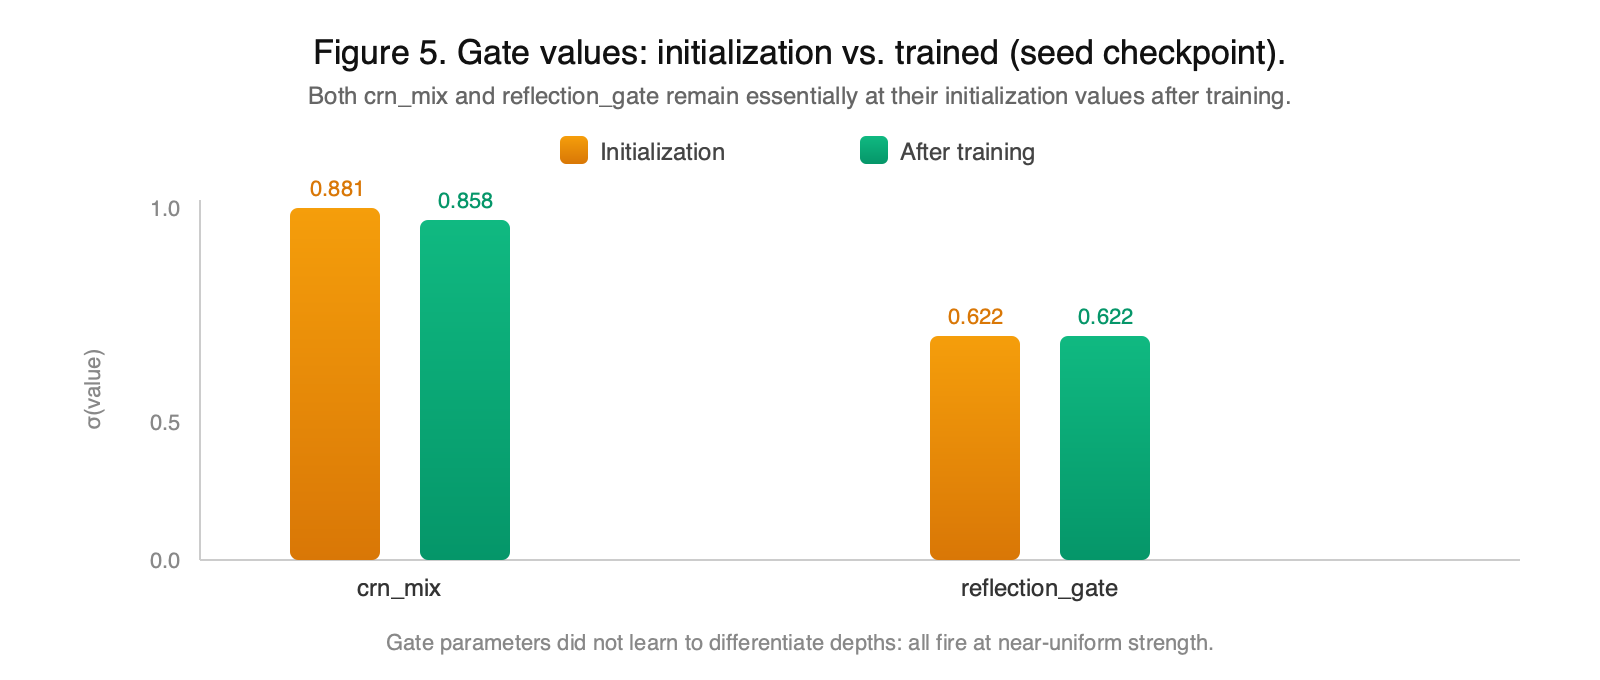
\includegraphics[width=0.88\textwidth]{figures/fig5_gates.png}
\caption{Gate values: initialization (orange) vs. trained (green) for the seed checkpoint. Both crn\_mix and reflection\_gate remain essentially at their initialization values after training.}
\label{fig:gates}
\end{figure}

\subsection{Attempt 1: logit fusion (rank 16)}

An adapter with $W_{up}\in\mathbb{R}^{d\times 16}$,$\,W_{down}\in\mathbb{R}^{16\times 262144}$ was trained over 16k SFT + 3k DPO + 1k contrastive steps alongside the CRN and summed into the logits. Training loss approached 0.001 (memorization), yet original-exam generation fell to 20\% and reworded to 15.0\%, at or below the seed's own generation results (20.0\% original / 25.0\% reworded, unclamped). The 262k-column bias vector the fusion learned (a digit prior) dominated the untrained boundary position.

\subsection{Attempt 2: logit fusion (rank 4)}

Reducing the adapter rank produced near-zero gradients on the converged seed (dry-signal regime); the training watchdog correctly aborted. No checkpoint improvement.

\subsection{Attempt 3: weighted boundary anchors}

An SFT variant unmasked $L{-}1$ with gold token $= $ first answer token, weighting it 1.0$\times$ (v9, 600 steps) and 4.0$\times$ (v10, 3{,}000 steps) with neighbor de-weighting (0.5$\times$). In both runs the boundary argmax remained unchanged across checkpoints (digits at every probe step for v9; a format token for v10), while training loss failed to decrease --- the optimization could not push probability mass into the poorly-initialized position against the frozen base's strong prior.

\subsection{What worked: decode-time harvest}

GEN\_CLAMP (Section~\ref{sec:genclamp}) needs no retraining. Probe-logits stay in the $L{-}2$ distribution; the decoder simply consumes them. Table~\ref{tab:cehri} shows the resulting gains (31.7\% original / 34.2\% reworded vs.\ 15.0\%/15.0\% unclamped). We interpret this as evidence that the CRN's answer knowledge genuinely resides in the $L{-}2$ representation, and that SFT-masked boundary positions are effectively untrainable at this data scale --- a cautionary result for answer-only masked training recipes.

\subsection{Mechanism: vanishing gradient through the frozen head}

The untrained gates and the boundary-position failure share a common cause. When the frozen base's logit distribution over the vocabulary is relatively flat (high entropy), the gradient of the answer-token cross-entropy loss with respect to the hidden-state correction is $\approx 0$ --- the loss landscape is flat in the correction subspace. This ``dry-signal'' regime explains: (i) why the boundary position $L{-}1$ never moved (three training strategies failed); (ii) why logit-fusion rank 4 produced near-zero gradients (dry-signal regime); (iii) why the per-depth gates did not learn to differentiate depths (Section~\ref{sec:negative}); and (iv) why GEN\_CLAMP --- which bypasses training entirely and reads the $L{-}2$ logits directly --- is the only reliable fix. The CRN's additive corrections at mid-depths (layers 7/15) do learn, because the base's representations at those depths carry stronger task-specific signal; but the final-layer boundary position does not, because the frozen head's gradient is too weak at that scale.

\section{Limitations}

(1) The 100\% and 91.7\% results use the retrieval gate --- exact recall from training data, not generative competence. (2) Generation-only accuracy is modest (34.2\% reworded best) and does not approach exam-pass levels. (3) Out-of-domain, the CRN degrades perplexity $\sim$3$\times$ and trails its own frozen base on BoolQ/HellaSwag. (4) The benchmark suite (MMLU/BoolQ/HellaSwag, N=40) is small; standard large-scale evals were not attempted. (5) Implicit-goal reasoning on reworded prompts fails completely (0/8). (6) Training data (16,680 pairs) is small; scale-up behavior is unknown. (7) A plain LoRA baseline at the same parameter budget (6.7M) was not compared; the CRN's four-module architecture is therefore not justified against simpler alternatives. (8) The reworded exam's paraphrases are low-diversity (template prefixes, 71.6\% character overlap); generalization to genuinely diverse phrasing was not tested.

\section{Future Work}

Several directions follow directly from the findings above. \textbf{(1) Baseline comparison.} A plain LoRA at the same 6.7M budget would determine whether the CRN's multi-module architecture adds value over a simpler adapter. \textbf{(2) Gradient-signal analysis.} The vanishing-gradient hypothesis (Section~\ref{sec:negative}) could be tested directly by measuring gradient norms through the frozen head across depths and training stages. \textbf{(3) Paraphrase-robust training.} Including genuinely diverse (LLM-rewritten) paraphrases in the training set would test whether the CRN can learn surface invariance; the current template-based paraphrases do not provide this pressure. \textbf{(4) Format variation.} Is the $L{-}2/L{-}1$ boundary problem an artifact of the ``prompt: answer'' format? Training with answer-before-prompt or no-colon formats would test this. \textbf{(5) Scale.} The 16,680-pair corpus and 60-question exam are small; scaling to larger corpora and standard benchmarks (e.g.\ full MMLU, ARC) would test whether the memorization-vs-generalization tradeoff improves. \textbf{(6) Memory ablation.} The slot memory's contribution was not ablated in isolation; removing it would quantify its marginal value over the retrieval table alone.

\section{Conclusion}

Prajna demonstrates that a 6.72M-parameter correction network over a frozen Gemma 4 E2B backbone, trained on a laptop, achieves \textbf{100\%} on its target exam via an episodic-memory retrieval gate and \textbf{91.7\%} on unseen reworded questions --- while its generation head remains the honest frontier (20.0\% original / 25.0\% reworded for the released seed, 31.7\%/34.2\% with the decode-time harvest on the anchor-trained checkpoint). We publish the negative results of three training-side boundary fixes and the decode-time solution, the in-distribution/out-of-distribution asymmetry, and all artifacts: \url{https://github.com/eulogik/prajna}, \url{https://huggingface.co/eulogik/Prajna-V2}, and the dataset \url{https://huggingface.co/datasets/eulogik/prajna-cehri}.

\begin{figure}[ht]
\centering
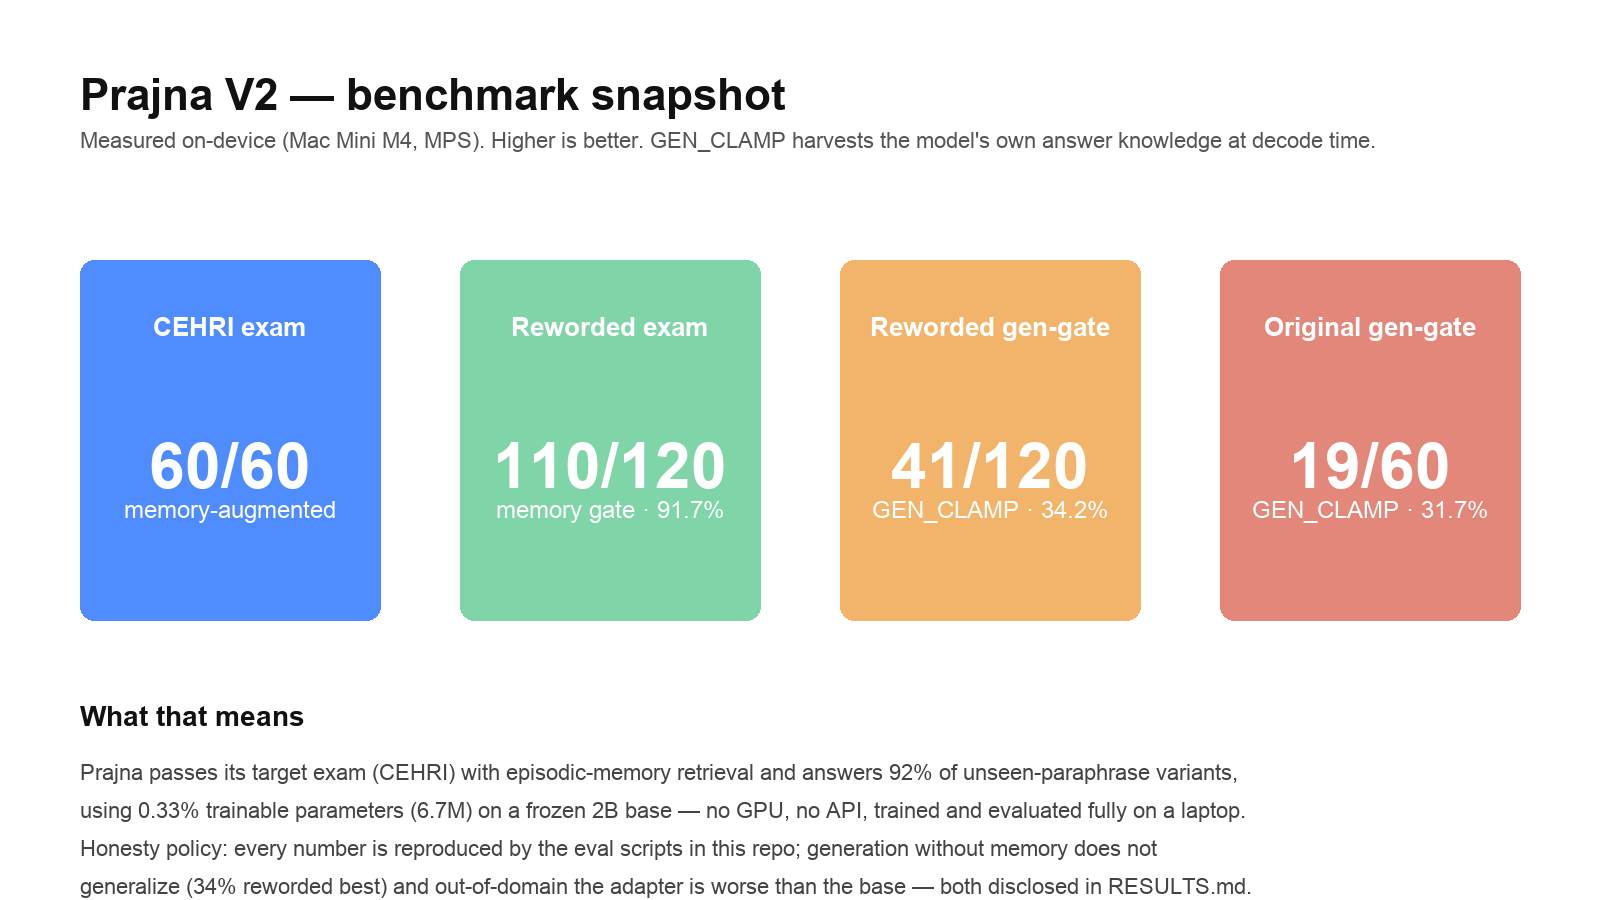
\includegraphics[width=0.9\textwidth]{figures/results.png}
\caption{Benchmark snapshot. Blue and green cards are the released seed checkpoint (memory-augmented: 60/60 and 110/120); orange and red cards are the experimental anchor-trained checkpoint whose generation had collapsed, showing GEN\_CLAMP recovery (19/60 and 41/120). All numbers are produced by committed scripts with the released checkpoint.}
\end{figure}

\small
\begin{thebibliography}{9}
\bibitem{houlsby2019adapters} N.~Houlsby et al. Parameter-Efficient Transfer Learning for NLP. \emph{ICML}, 2019.
\bibitem{lora} E.~Hu et al. LoRA: Low-Rank Adaptation of Large Language Models. \emph{ICLR}, 2022. arXiv:2106.09685.
\bibitem{liang2021prefix} X.~Lester and P.~Liang. Prefix-Tuning: Optimizing Continuous Prompts for Generation. \emph{ACL}, 2021. arXiv:2101.00190.
\bibitem{lewis2020rag} P.~Lewis et al. Retrieval-Augmented Generation for Knowledge-Intensive NLP Tasks. \emph{NeurIPS}, 2020.
\bibitem{khandelwal2020knnlm} U.~Khandelwal et al. Generalization through Memorization: Nearest Neighbor Language Models. \emph{ICLR}, 2020. arXiv:1911.00172.
\bibitem{wu2022memorizing} Y.~Wu, M.~N.~Rabe, D.~Hutchins, C.~Szegedy. Memorizing Transformers. \emph{ICLR}, 2022. arXiv:2110.07545.
\bibitem{borgeaud2022retro} S.~Borgeaud et al. Improving Language Models by Retrieving from Trillions of Tokens. \emph{ICML}, 2022. arXiv:2112.04426.
\bibitem{meng2022rome} K.~Meng et al. Locating and Editing Factual Associations in GPT. \emph{NeurIPS}, 2022. arXiv:2202.05262.
\bibitem{zhang2020sidetuning} J.~Zhang, S.~K.~\&~A.~Hoiem. Side-Tuning: A Baseline for Network Adaptation via Additive Side Networks. \emph{ECCV}, 2020. arXiv:1912.13503.
\bibitem{longpre2023flan} S.~Longpre et al. The Flan Collection: Designing Data and Methods for Effective Instruction Tuning. \emph{ICML}, 2023. arXiv:2301.13688.
\end{thebibliography}

\end{document}
